\documentclass[a4paper,13pt]{article}
\usepackage[T1]{fontenc}
\usepackage[utf8x]{inputenc}
\usepackage[italian,english]{babel}
\usepackage{lipsum}
\usepackage{url}
\usepackage{graphicx}
\begin{document}
\author{Andrea Pagliaro , Alessio Susco \and Shanj Zaccaretti}
\title{Studio e Progettazione del controllo sulla velocita di rotazione di un gneratore eolico}
\maketitle
\section{Introduzione}
Per lo studio e la progettazione di un controllore lineare che regoli la rotazione di una turbina eolica in modo che sia costante mediante il pitch , sono state prese in considerazione varie equazioni riguardanti il moto di un rotore e le relative potenze ricavate.
Come le seguenti :
\begin{equation}
P=\frac{1}{2}\,\rho\,A\,C_p\,V_w^3
\end{equation}
Che rappresenta la quantit\'a di potenza assorbita dal rotore della turbina eolica presa in considerazione.
Il Cp \'e il coefficiente di potenza dipendente da $\lambda$ e $\beta$.
Dove a loro volta $\lambda$ \'e dato da :
\begin{equation}
\lambda=\frac{\Omega\,R}{V_w}
\end{equation}
Che viene chiamato tip-speed ratio ed \'e dato dal rapporto tra la velocita angolare
del rotore per il suo raggio e la velocita del vento.
Mentre $\beta$ rappresenta l'angolo di pitch relativo alle pale.
Chiaramente la funzione del coefficiente di potenza comporta delle dinamiche non 
lineari dipendenti dalla geometria del rotore questo a sua volta si ripercuote sull'intero sistema che lo rende non lineare.  
Ora provando a linearizzare il sistema ci \'e risultato molto difficile e solo dopo aver letto alcune pubblicazioni sullo studio di turbine eoliche siamo riusciti a trovare alcune linearizzazioni compiute mediante metodi numerici, che ci hanno permesso di riscrivere il sistema nella seguente forma:
\begin{equation}
\dot{x_1}=\frac{\gamma}{I_{rot}}\,x_1+\frac{\sigma}{I_{rot}}\,\delta_\beta+\frac{\alpha}{I_{rot}}\,\delta_\omega
\end{equation}
Dove x_1 , lo stato del sistema rappresenta la velocita angolare del rotore ,
$\delta_\beta$ \'e l'ingresso relativo alla perturbazione da parte del pitch,
$\delta_\omega$ \'e la perturbazione realtiva alla velocita del vento.
Quindi la nostra matrice di stato \'e data da $A=\frac{\gamma}{I_{rot}}$,
e i coefficienti dei rispettivi ingressi:
$B=\frac{\sigma}{I_{rot}}$
$\Gamma=\frac{\alpha}{I_{rot}}$
Irot rappresenta inerzia del rotore.
I valori $\gamma$ , $\sigma$ , $\alpha$ rappresentano le derivate parziali ricavate attraverso 
l'equazione dell'aerodinamica del rotore descritta in tal modo:
\begin{equation}
T_{aero}=T(\omega_0,\Omega_0,\beta_0)+\frac{\delta \, T_{aero}}{\delta \, \Omega}+
\frac{\delta \, T_{aero}}{\delta \, \beta}+\frac{\delta \, T_{aero}}{\delta \, \omega}
\end{equation} 
Dove i coefficienti $\gamma=\frac{\delta \, T_{aero}}{\delta \, \Omega}$=-0.1205
$\sigma=\frac{\delta \, T_{aero}}{\delta \, \beta}$=-2.882,
$\alpha=\frac{\delta \, T_{aero}}{\delta \, \omega}$=0.0658
sono gia noti essendo stati ricavati dalla linearizzazione eseguita mediante un metodo numerico non descritto nella pubblicazione di cui si sta facendo uso per il progetto in questione.
I valori degli stati iniziali sono dati da $\omega_0$=18m/s , $\Omega_0$=42RPM e $\beta_0$=12deg.
Detto questo siamo passati alla progettazione del controllore, ed \'e stato scelto un controllo con guadagno proporzionale per il momento.
Successivamente si proceder\'a ad inserire i i guadagni giusti per un controllo proporzionale-integrativo(PI).
Lo schema del sistema con relativo controllo e circuito di gestione per l'event triggering (estratto dal SIMULINK di matlab).
\begin{center}
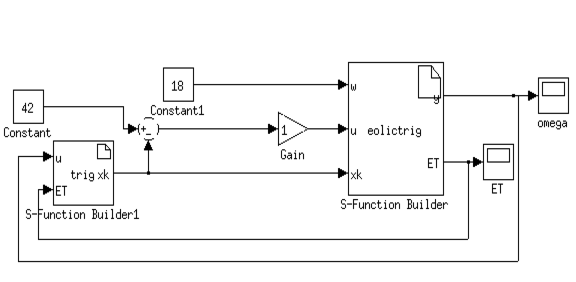
\includegraphics[scale=0.6]{schema1.png}
\end{center}
Per quanto riguarda le tecniche di controllo per l'event-triggering ,\'e stato inserito un sistema che riceve l'uscita del nostro processo e il valore del trigger che viene calcolato all'interno dello stesso e che quindi effettua un cambio dello stato solo quando viene commutato il trigger.Avendo fatto le opportune ipotesi , l'intero sistema prima di essere descritto anche in SIMULINK \'e stato simulato attraversato il SIMNON.
I risultati riportati dalla simulazione per velocita del vento=18 e velocita di rotazione del rotore=42(riferimento) sono i seguenti.
\begin{center}
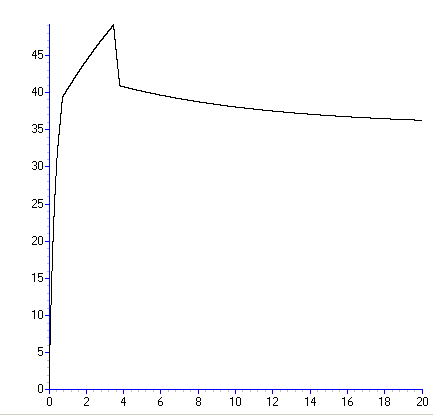
\includegraphics[scale=0.6]{PLOT_OMEGA.png}
\end{center}
Dove in questo grafico \'e mostrato l'andamento dell'uscita ovvero del velocita di rotazione del rotore che partendo da 0 raggiunge i 42 RPM in 20 secondi di simulazione.
Si possono notare i picchi dovuti alla commutazione del trigger.
\begin{center}
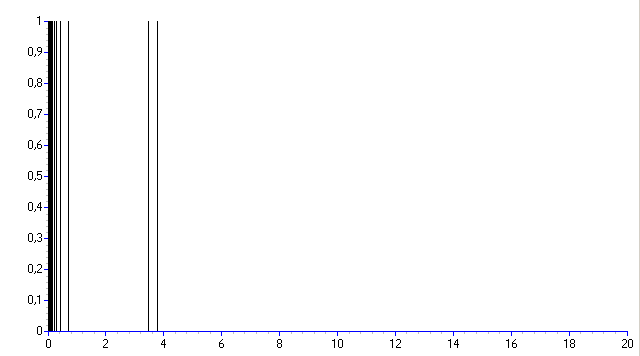
\includegraphics[scale=0.6]{PLOT_ET.png}
\end{center}
Nel seguente invece si sta facendo riferimento alle commutazioni avvenute nell'arco di 20 secondi.
\begin{center}
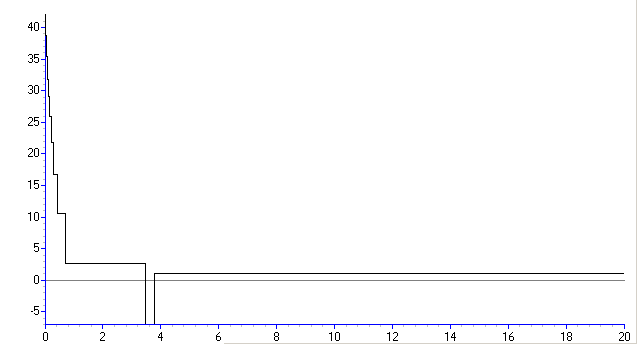
\includegraphics[scale=0.6]{PLOT_UD.png}
\end{center} 
L'ultimo grafico mostra un segnale discreto che e' proprio l'ingresso del nostro processo in seguito alla controreazione ottenuta dopo un controlo di tipo proporzionale e dipendente dal trigger di fatto  risulta essere un segnale discreto aperiodico.
Per quanto riguarda il sistema generale mancano ancora i calcoli da effettuare per i coefficienti da inserire per il controllo dell'event-triggering poiche sono solo di prova ed utilizzati per la simulazione come anche quelli del guadagno proporzionale.
\end{document}


